% Written by
% Omur Ugur
% Email: ougur@metu.edu.tr
%
% can be any class (with options) hopefully
% a4paper and 12pt options are not mandatory, but preferred 
\documentclass[a4paper, 12pt]{article} % for a simple paper
%\documentclass[a4paper, 12pt]{report} % for a term project

% Language Specific (generally not neede):
%\usepackage[T1]{fontenc} 
%\usepackage[utf8]{inputenc}
% it is important that you load this package: iamPaperStyle.sty
\usepackage{iamPaperStyle} %includes also graphicx.sty and xcolor.sty

% any other styles you need
% not mandatory, but helful 
\usepackage{graphicx} % although loaded by iamPaperStyle.sty
\usepackage{wrapfig}
\usepackage{amsmath, amssymb, amsthm} % others
\usepackage{hyperref} % other

% you may use a bit larger area on an a4paper in the document by
\usepackage{a4wide} % not necessary but generally useful
\usepackage{caption}
\usepackage{subcaption}
\usepackage[ruled,vlined]{algorithm2e} % package for algorithms.
\usepackage{amsmath,amsfonts}

% now you may begin
\begin{document}

\studentName{Uğurcan Özalp}
\advisorName{Prof.~Dr.~Ömür Uğur}
% Your Department: 
% Scientific Computing, 
% Financial Mathematics, 
% Cryptography, or 
% Actuarial Sciences
\departmentName{Scientific Computing}
% Type of the Document:
% Preprint # may not work as expected (to-do)
% Qualification in PhD
% Report for Thesis Monitoring Committee
% Term Project
% Draft of a Manuscript
\paperType{Draft of a Manuscript}


\paperTitle{%
	Bipedal Robot Walking by Reinforcement Learning in Partially Observed Environment
}

\paperAuthor{%
  U. \"{O}zalp\footnote{%
    Middle East Technical University, Institute of Applied
    Mathematics, 06800 \c{C}ankaya, Ankara, Turkey. \hfill
  \emph{E-Mail}: \texttt{ugurcan.ozalp@metu.edu.tr}},
	% possibly your advisor and co-advisor
  \"{O}. U\u{g}ur\footnote{Middle East Technical University, Institute of Applied
  Mathematics, 06800 \c{C}ankaya, Ankara, Turkey. \hfill
  \emph{E-Mail}: \texttt{ougur@metu.edu.tr}}
}
% abstract should not be large to fit in the title/front page
\paperAbstract{%
Deep Reinforcement Learning methods on mechanical control have been successfully applied in many environments and used instead of traditional optimal and adaptive control methods for some complex problems. 
However, Deep Reinforcement Learning algorithms do still have some challenges. 
One is to control on partially observable environments. 
When an agent is not informed well of the environment, it must recover information from the past observations. 
In this thesis, walking of Bipedal Walker Hardcore (OpenAI GYM) environment, 
which is partially observable, 
is studied by two continuous actor-critic reinforcement learning algorithms; Twin Delayed Deep Determinstic Policy Gradient and Soft Actor Critic.
Several neural architectures are implemented. 
The first one is Residual Feed Forward Neural Network under the observable environment assumption, 
while the second and the third ones are Long Short Term Memory and Transformer using observation history as input to recover the hidden information due to the partially observable environment. 
}

\paperKeywords{%
  deep reinforcement learning, partial observability, robot control, actor-critic methods, long short term memory, transformer
}

\paperDate{July 2021}

 % edit this file or see the lines below
%%%%%%%%%%%%%%%%%%%%%%%%%%%%%%%%%%%%%%%%%%%%%%%%%%%%%%%%%%%%%%%%%%%%%
% you may also use the predefined macros also here to over-write the
% info in the included file newPreprintDetails.tex

% \studentName{Ömür Uğur}
% \advisorName{Prof.~Dr.~Hamdullah Yücel}
% \departmentName{Scientific Computing}
% \paperType{Draft of a Manuscript}
% \paperTitle{This is the Title}
% \paperAuthor{\"{O}. U\u{g}ur, A. Mehmet}
% \paperAbstract{This is the Abstract} 
% \paperKeywords{Keyword 1, no keyword, illegalWord}
% \paperDate{April 2013} 

%%% mandatory:
\makePaperCoverPage
% for printing (and submitting) uncomment below (to have a sigle title page)
%\blankpage
%%%%%%%%%%%%%%%%%%%%%%%%%%%%%%%%%%%%%%%%%%%%%%%%%%%%%%%%%%%%%%%%%%%%%


%%%%%%%%%%%%%%%%%%%%%%%%%%%%%%%%%%%%%%%%%%
% The rest of the manuscript is trivial...
%%%%%%%%%%%%%%%%%%%%%%%%%%%%%%%%%%%%%%%%%%
% Hoever, try not to use commands like
% \title, \author, \date, \maketitle or \tableofcontents
% unless you need them of course: 
% you might need a title and a table of contents
% at the begining sometimes
%\title{Title of the Manuscript}
%\author{Author Name Surname}
%\date{\today}
%\maketitle

% if necessary (suggested in a simple paper submitted to IAM}
\makeTitle % don't use this if this is a term project
\tableofcontents % will be a separate page in case of term project


%%%%%%%%%%%%%%%%%%%%%%%%%%%
% CONTENT OF THE MANUSCRIPT
%%%%%%%%%%%%%%%%%%%%%%%%%%%

% instead of typing here inside this document
% we suggest you to include or input a
% separate document of yours:
% \input{yourdocname}

% For Reports un comment \chapter{}
%\chapter{In case of a Report Chapter is needed}
%		\label{chap:ReportIntro}

\section{Introduction} \label{sec:first_intro}

Humans and animals exhibit several different behaviours in terms of 
interaction with environment, such as utterance and movement. 
Their behavior is based on past experience, the situation they are in  and their objective. 
Like humans and animals, an intelligent agent is expected to take 
action according to its perception based on some objective. 
A major challenge in Machine Learning to create agents that will 
act more natural and humanlike. 
As a subfield of ML, Reinforcement Learning (RL) allows an 
agent to learn how to control (or act) itself in different situations by interacting with the environment. In RL, environment is modeled to give reward (or punishment) to agent 
according to environmental state and agent actions, and agent focuses
on learning to predict what actions will lead to highest reward 
(or lowest punishment, based on its objective) in the future using past experience. 

Traditional RL algorithms need feature engineering from observations. 
For complex problems, the way to extract features is ambiguous or 
observations are not enough to create a good model. 
In contrast to traditional methods, Deep Neural Networks (DNNs) allows to extract 
high level features from data with large state-space 
(pixelwise visual, many kinematic sensors etc.) and missing  observations.
Along with recent developments in DNNs, Deep Reinforcement Learning (DRL)
allows an agent to interact with the environment in a more complex way.

Since its discovery, robots have been crucial devices for the human race, whether smart or not. 
Intelligent humanoid and animaloid robots have been developed since early 1980s. 
This type of robots has legs unlike driving robots. 
Since most of the world terrain is unpaved, this type of robots are good alternative to driving robots. 
Locomotion is a major task for such robots. Stable bipedal (2 legged)  walking 
is one of the most challenging problem among the control problems. 
It is hard to create accurate model due to high order of dynamics,  friction and discontinuities. 
Even further, the design of walking controller using traditional methods is difficult due to the same reasons. 
Therefore, for bipedal walking, DRL approach is an easier choice if a simulation environment is available. 

In this work, Bipedal Locomotion is investigated through \textit{BipedalWalker-Hardcore-v3} \cite{noauthor_bipedalwalkerhardcore-v2_2021} environment of open source GYM library \cite{brockman_openai_2016} by DRL. 
Our contributions are as follows:
\begin{itemize}
	\item Sequential neural networks are used (LSTM and Transformer) for solution, along with Residual Feed Forward Neural Network.
	\item Twin Delayed Deep Deterministic Policy Gradient (TD3) and Soft Actor-Critic (SAC) algorithms are used and compared.
	\item Reward shaping and small modifications are applied on environment to hinder possible problems.
\end{itemize}

\section{Environment Details}

\subsection{Dynamics}

\textit{BipedalWalker} environments~\cite{noauthor_bipedalwalker-v2_2021, noauthor_bipedalwalkerhardcore-v2_2021} are parts of Gym environment library. 
One of them is classical where the terrain is relatively smooth, while other is a hardcore version containing ladders, stumps and pitfalls in terrain. 
However, terrain is randomly generated at the beginning of each episode.
Dynamics of the robot are exactly identical in both environments. 
The robot has kinematic and lidar sensors. 
It is modeled as Markov Decision Process with deterministic dynamics.

Those environments have continuous action and observation space. 
\textbf{Observation Space} contains hull angle, hull angular velocity, hull translational velocities, joint positions, joint angular speeds, leg ground concats and ten lidar rangefinder measurements.
The robot has 2 legs with 2 joints at knee and hip. Torque provided to knee and pelvis joints of both legs. These 4 torque values forms  \textbf{Action Space}.

\textbf{Reward Function} is designed to move the robot forward as much as possible.
The robot should run fast with little energy while not stumble and fall to ground. 
Directly proportional to distance traveled forward, +300 points given if agent reaches end of path. 
-10 points (-100 points in original version) if agent falls, 
and small amount of negative reward proportional to applied motor torque (to prevent applying unnecessary torque). 
Lastly, the robots gets negative reward propotional to absolute value of hull angle for reinforcing to keep hull straigth. 

Snapshots for both environments are depicted in Figure \ref{fig:bipedal_walkers}.

\begin{figure}
	\begin{subfigure}{.5\textwidth}
		\centering
		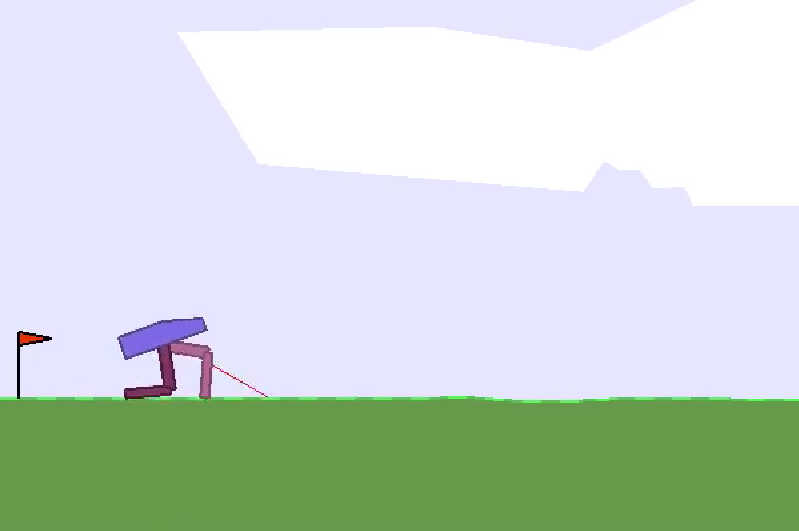
\includegraphics[width=0.9\linewidth]{figures/bipedal/classic.png}
		\caption{BipedalWalker-v3 Snapshot~\cite{noauthor_bipedalwalker-v2_2021}}
		\label{fig:bipedal_walker_classic}
	\end{subfigure}
	\begin{subfigure}{.5\textwidth}
		\centering
		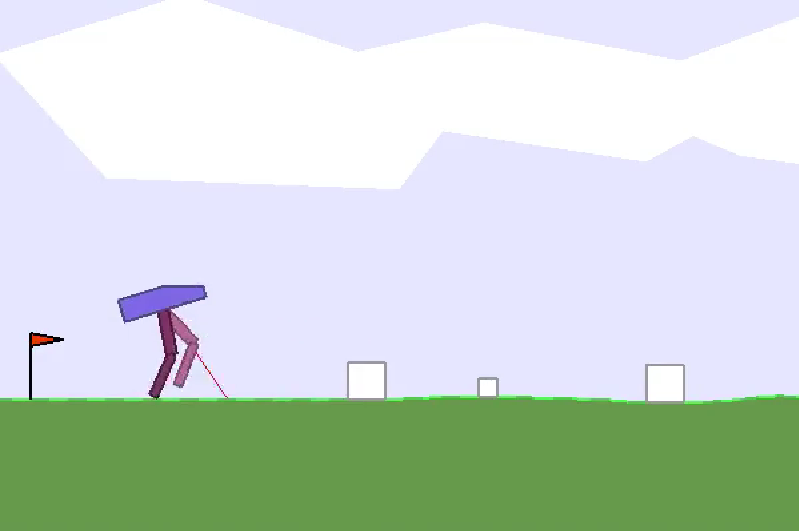
\includegraphics[width=0.9\linewidth]{figures/bipedal/hardcore.png}
		\caption{BipedalWalkerHardcore-v3 Snapshot~\cite{noauthor_bipedalwalkerhardcore-v2_2021}}
		\label{fig:bipedal_walker_hardcore}
	\end{subfigure}
	\caption{Bipedal Walkers Snapshots}
	\label{fig:bipedal_walkers}
\end{figure}

\subsection{Difficulties}

Locomotion of the Bipedal Walker is a difficult control problem due to following reasons: 
\begin{itemize}
	\item \textbf{Nonlinearity}: The dynamics are nonlinear, unstable and multimodal. 
	Dynamical behavior of robot changes for different situations 
	like ground contact, single leg contact and double leg contact.
	\item \textbf{Uncertainity}: The terrain where the robot walks also varies. 
	Designing a controller for all types of terrain is difficult.
	\item \textbf{Reward Sparsity}: Overcoming some obstacles requires a specific maneuver, which is hard to explore sometimes.	
	\item \textbf{Partially Observability}: The robot observes 
	ahead with lidar measurements and cannot observe behind, as illustrated in Figure \ref{eqn:partial_obs_pitfall}. 
	In addition, it lacks of acceleration sensors.
\end{itemize}

\begin{figure}
	\begin{subfigure}{.32\textwidth}
		\centering
		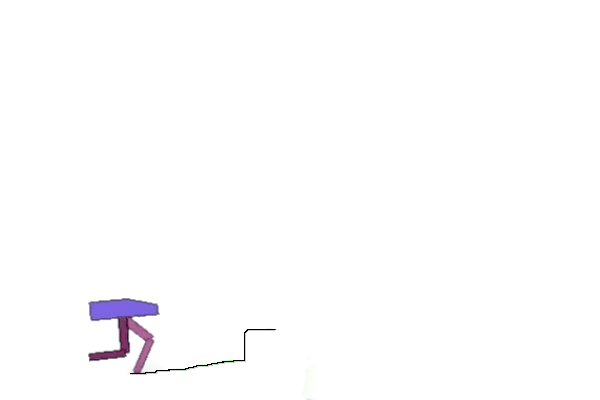
\includegraphics[width=0.99\linewidth]{figures/bipedal/po/lidarcover.png}
		\caption{Perspective}
		\label{fig:lidar_cover}
	\end{subfigure}
	\begin{subfigure}{.32\textwidth}
		\centering
		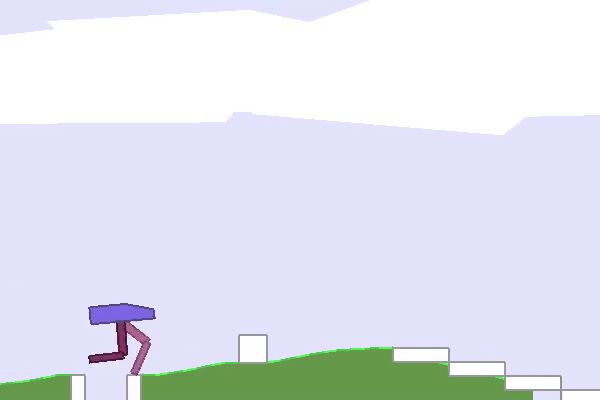
\includegraphics[width=0.99\linewidth]{figures/bipedal/po/pitfall_behind.png}
		\caption{Pitfall Behind}
		\label{fig:pitfall_behind}
	\end{subfigure}
	\begin{subfigure}{.32\textwidth}
		\centering
		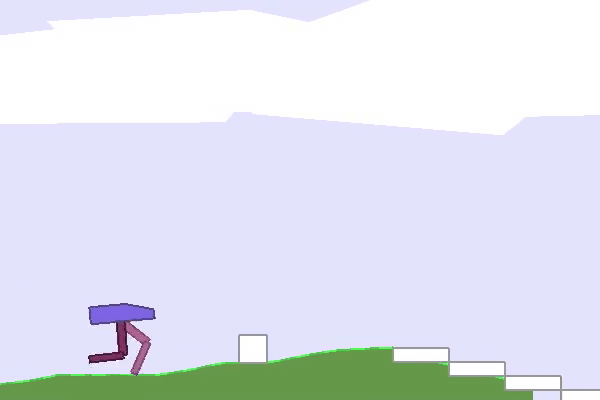
\includegraphics[width=0.99\linewidth]{figures/bipedal/po/no_pitfall_behind.png}
		\caption{No Pitfall Behind}
		\label{fig:no_pitfall_behind}
	\end{subfigure}
	\caption{Perspective of agent and possible realities}
	\label{fig:partial_obs_pitfall}
\end{figure}

These reasons make it also hard to implement analytical methods for control tasks. 
However, DRL approach can easily overcome nonlinearity and uncertainity problems.

On the other hand, reward sparsity problem brings local minimums to objective function of optimal control. However, this can be challenged by a good exploration strategy and reward shaping. 

For the partial observability problem, more elegant solution is required. 
This is, in general, achieved by creating a belief state from the past observations to inform the agent. 
Agent uses this belief state to choose how to act. 
If the belief state is evaluated sufficiently, 
this increases performance of the agent.
Relying on instant observations is also possible, 
and this may be enough sometimes if advanced type of control is not required. 

\section{Reinforcement Learning}

\textbf{Reinforcement Learning} is the closest kind of learning demonstrated by humans and animals 
since it is grounded by biological learning systems. 
It is based on maximizing cumulative reward over time to make agent 
learn how to act in an environment~\cite{sutton_reinforcement_1998}. 
Each action of the agent is either rewarded or punished according to a reward function. 
The agent explores environment by taking various actions in different states to gain experience, based on trial-and-error. 
Then it exploits experiences to get highest reward from the environment considering instant and future rewards over time. 

RL is a stochastic control process. 
At time $t$, the agent starts with state $s_t \in \mathcal{S}$ and observes $o_t \in \mathcal{O}$, 
then it takes an action $a_t \in \mathcal{A}$ according to its policy $\pi$ and obtains a reward $r_t \in \mathbb{R}$ at time $t$. 
Hence, a state transition to $s_{t+1} \in \mathcal{S}$ occurs as a consequence of the action and the agent gets the next observation $o_{t+1} \in \mathcal{O}$. 
Along with state transitions, the agent is expected to develop (learn) a policy function 
$\pi \colon \mathcal{S} \rightarrow \mathcal{A}$ which maps 
inputs (observations) $s \in \mathcal{S}$ to outputs (actions) $a \in \mathcal{A}$ to maximize rewards over time.

\subsection{Policy Learning}

Policy learning is achieved by maximization of the action value function, which is expected cumulative sum of future rewards scaled by discount factor $\gamma$. Action value function is defined as follows;
\begin{equation}
Q^{\pi}(s,a) = \mathbb{E}\bigg[\sum_{i=t}^{\infty} \gamma^{i-t} r_i|s_t=s, a_t=a, \pi\bigg]. %\quad \forall t = 0,1, ...
\end{equation}
for all possible states and actions. 
Bellman proved that optimal value function, for a model $T$, should satisfy following conditions~\cite{bellman_dynamic_2003}. 
\begin{equation}
\label{eqn:bellman_q}
Q^{*}(s,a) = \mathbb{E}[r|s,a] + \gamma \max_{a'} \Big\{ \sum_{s'} T(s'|s,a) Q^{*}(s',a') \Big\}
\end{equation}
Most of RL methods are build upon solving \eqref{eqn:bellman_q}, since there exist a direct relation between $Q^*$ and $\pi^*$, which is 
\begin{equation}
\label{eqn:policy_stochastic_q}
\pi^{*}(a|s) = 
\begin{cases}
1,   & \text{if  } a = \arg\max_{a} Q^{*}(s,a), \\
0,   & \text{otherwise  }.
\end{cases} 
\end{equation}

\subsection{Q Learning}
Q Learning is based on optimizing $Q$ function using Bellman Equation \eqref{eqn:bellman_q}~\cite{watkins_technical_1992}. 
In this learning strategy, $Q$ function is assumed to be parametrized by $\theta$. 
Target $Q$ value is estimated by bootstrapping estimate, 
\begin{equation}
\label{eqn:q_target}
Y_t^Q = r_t + \gamma \max_{a'} Q(s_{t+1},a';\theta).
\end{equation}
At time $t$,  with state, action, reward, next state tuples ($s_t,a_t,r_t,s_{t+1}$), 
$Q$ values are updated by minimizing difference between the target value and the estimated value. 
Hence the loss 
\begin{equation}
\label{eqn:q_loss}
\mathcal{L}_t(\theta) = \big( Y_t - Q(s_t,a_t;\theta) \big) ^ 2, 
\end{equation}
is to be minimized with respect to $\theta$ using numerical optimization methods. 

\subsection{Deep Q Learning}
When a nonlinear approximator is used for $Q$ estimation, learning is unstable due to the correlation among recent observations. 
Deep Q Learning solves this problem by introducing Target Network and Experience Replay \cite{mnih_human-level_2015, mnih_playing_2013} along with using deep neural networks. 

\textbf{Target Network} is parametrized by $\theta^-$. 
It is used to evaluate target value, but it is not updated by the loss minimization. 
It is updated at each fixed number of update step by Q network parameter $\theta$. 
In this way, correlation between target value and observations are reduced.
The target value is obtained by using $\theta^-$ as
\begin{equation}
\label{eqn:dqn_ntarget}
Y_t^{DQN} = r_t + \gamma \max_{a'} Q(s_{t+1},a';\theta^-).
\end{equation}

\textbf{Experience Replay} stores experience tuples in the replay memory $\mathcal{D}$ as a queue with fixed buffer size $N_{replay}$. 
At each iteration $i$, $\theta$ is updated by experiences $(s,a,r,s')\sim U(\mathcal{D})$ uniformly subsampled from experience replay by minimizing the expected loss
\begin{equation}
\label{eqn:dqn_loss}
\mathcal{L}_i(\theta_i) = \mathbb{E}_{(s,a,r,s')\sim U(\mathcal{D})}\Big[\big( Y^{DQN} - Q(s,a;\theta_i) \big) ^ 2 \Big].
\end{equation}
It allows agent to learn from experiences multiple times at different stages of learning. 
More importantly, sampled experiences are close to be independent and identically distributed if buffer size is large enough. 
Again, this reduces correlation between recent observations and updated $Q$ value. This makes learning process more stable. 

\textbf{Epsilon Greedy Exploration} is used to let agent explore the environment. 
In discrete and finite action space $\mathcal{A}$, this is the simplest exploration strategy used in RL algorithms.
During the learning process, a random action with probability $\epsilon$, or greedy action (maximizing Q value) with probability $1-\epsilon$ is selected. 
In order to construct policy:   
\begin{equation}
\label{eqn:egreedy_policy}
\pi(a|s) = 
\begin{cases}
1-\epsilon,   & \text{if } a = \arg \max_{a} Q(s, a), \\
\frac{\epsilon}{|\mathcal{A}|-1},     & \text{otherwise},
\end{cases}
\end{equation}
where $|\mathcal{A}|$ denotes cardinality of $\mathcal{A}$. 

\subsection{Deep Deterministic Policy Gradient}
DDPG is continuous complement of DQN using a deterministic policy~\cite{lillicrap_continuous_2019}. 
It also uses experience replay and target networks. 
Similar to Deep Q Learning, there are target networks parametrized by $\theta^{\mu^-}$ and $\theta^{Q^-}$ 
along with the main networks parametrized by $\theta^{\mu}$ and $\theta^{Q}$. 

While target networks are updated in a fixed number of steps in DQN, 
DDPG updates target network parameters at each step with Polyak averaging, 
\begin{equation}
\label{eqn:target_update}
\theta^- \leftarrow \tau \theta + (1-\tau) \theta^- .
\end{equation}
The $\tau$ is an hyperparameter indicating how slow the target network is updated and it is usually close to zero. 

Policy network parameters are learned by maximizing resulting expected value, or minimizing its negative,
\begin{equation}
\label{eqn:ddpg_policy_loss}
\mathcal{L}_i(\theta^\mu_i) = -\mathbb{E}_{s \sim U(\mathcal{D})} \Big[ Q(s, \mu(s\theta^\mu_i);\theta^Q) \Big].
\end{equation} 
Note that value network parameters are also assumed to be learned. 

In addition, target networks are used to predict target value and the target is defined by 
\begin{equation}
\label{eqn:ddpg_target}
Y_t^{DDPG} = r_t + \gamma Q(s_{t+1}, \mu(s_{t+1};\theta^{\mu^-});\theta^{Q^-}).
\end{equation}
In each iteration, this target is used to learn $Q$ function by minimizing the least squares loss 
\begin{equation}
\label{eqn:ddpg_loss}
\mathcal{L}_i(\theta^Q_i) = \mathbb{E}_{s,a,r,s'\sim U(\mathcal{D})}\Big[\big( Y^{DDPG} - Q(s,a;\theta^Q_i) \big) ^ 2 \Big].
\end{equation}

In DDPG, value and policy network parameters are learned simultaneously. 
During the learning process, exploration noise is added to each selected action. 
In ~\cite{lillicrap_continuous_2019}, authors proposed to use Ornstein-Uhlenbeck Noise~\cite{uhlenbeck_theory_1930} in order to have temporal correlation for efficiency. 
However, a simple Gaussian white noise or any other one is also possible. 

\subsection{Twin Delayed Deep Deterministic Policy Gradient}
TD3~\cite{fujimoto_addressing_2018} is an improved version of DDPG with higher stability and efficiency. 
There are three main tricks upon DDPG: 

\textbf{Target Policy Smoothing} is to regularize the learning process by smoothing effects of actions on value. For target value assessing, actions are obtained from the target policy network in DDPG, while a clipped zero-centered Gaussian noise is added to actions in TD3 as follows: 
\begin{equation}
\label{eqn:td3_target_action}
\widetilde{a}' = \mu(s';\theta^{\mu^-}) + \text{clip}(\epsilon, -c, c), \quad \epsilon \sim \mathcal{N}(0, \sigma^2).
\end{equation}

\textbf{Clipped Double Q Learning} is to escape from $Q$ value overestimation. 
There are two different value networks with their targets. 
During learning, both networks are trained by single target value assessed by using whichever of the two networks give smaller. 
In other words, 
\begin{equation}
\label{eqn:td3_target}
Y_t^{TD3} = r_t + \gamma \min_{k\in\{1,2\}} Q(s_{t+1}, ;\widetilde{a}_{j+1};\theta^{Q_k^-}).
\end{equation}
On the other hand, the policy is learned by maximizing the output of the first value network, or minimizing its negative,
\begin{equation}
\label{eqn:td3_policy_loss}
\mathcal{L}_i(\theta^\mu_i) = -\mathbb{E}_{s \sim U(\mathcal{D})} \Big[ Q(s, \mu(s;\theta^\mu_i);\theta^{Q_1}) \Big].
\end{equation} 

\textbf{Delayed Policy Updates} is used for stable training. 
During learning, policy network and target networks are updated less frequently (at each fixed number of steps) than the value network. 
Since the policy network parameters are learned by maximizing the value network, they are learned slower.  

\subsection{Soft Actor-Critic}
SAC~\cite{haarnoja_soft_2018} is a stochastic actor-critic method and many characteristics are similar to TD3 and DDPG. Its main advantage is that it learns to maximize exploration with entropy regularization. 

SAC is an entropy-regularized RL method. Such methods give bonus reward to the agent propotional to the policy entropy: given state $s$, the entropy of a policy is defined by
\begin{equation}
\label{eqn:policy_entropy}
H(\pi(\cdot|s)) = \mathbb{E}_{\widetilde{a}\sim\pi(\cdot|s)}[-\log(\pi(\widetilde{a}|s))]
\end{equation}

Given the entropy coefficient $\alpha$, definition of state-action value function is redefined as follows: 
\begin{equation}
\label{eqn:q_dfn_entreg}
Q^{\pi}(s,a) = \mathbb{E}_{\substack{s'\sim T(\cdot|s,a)\\\widetilde{a}'\sim \pi(\cdot|s')} } \Big[r + \gamma \Big(Q^{\pi}(s',\widetilde{a}') -\alpha\log(\pi(\widetilde{a}'|s') \Big) \Big]. %\quad \forall t = 0,1, ...
\end{equation}

This modification changes $Q$ value target definition,
\begin{equation}
\label{eqn:q_target_sac}
Y_t^{SAC} = r_t + \gamma \Big(\min_{k\in\{1,2\}} Q(s_{t+1}, ;\widetilde{a}_{t+1};\theta^{Q_k^-}) -\alpha\log(\pi(\widetilde{a}_{t+1}|s_{t+1})) \Big),
\end{equation}
where $\widetilde{a}_{t+1} \sim \pi(\cdot|s_{t+1}; \theta^{\pi})$.

While the policy is updated according to first value network by \eqref{eqn:td3_policy_loss} in TD3, the policy is updated according to minimum value of both networks output along with the entropy regularization, 
\begin{equation}
\label{eqn:sac_policy_loss}
\mathcal{L}_i(\theta^\pi_i) = - \mathbb{E}_{\substack{s \sim U(\mathcal{D})\\\widetilde{a} \sim \pi(\cdot|s)}} \Big[ \min_{k\in\{1,2\}} Q(s, \widetilde{a};\theta^{Q_k^-}) - \alpha\log(\pi(\widetilde{a}|s;\theta^\pi_i)) \Big].
\end{equation}

The policy function is stochastic in SAC, and in practice, it is a parametrized probability disribution. Most common one is 
Squashed Gaussian policy to squash actions in the range $(-1,1)$ by $\tanh$ function. 
This is parametrized by its mean and standart deviation, i.e., $\theta^{\pi}=(\theta^{\mu}, \theta^{\sigma})$. Actions are then sampled as follows: 
\begin{equation}
\label{eqn:squashed_gp_sampling}
a(s) = \tanh(\mu(s; \theta^{\mu}) + \eta \odot \sigma(s; \theta^{\sigma})), \quad \eta \sim \mathcal{N}(0, I), 
\end{equation}
where $\odot$ is elementwise multiplication.

Finally, we note that SAC method does not include policy delay, target policy smoothing and target policy network. 

\section{Methodology}

\subsection{Modifications on Original Envrionment}

It is difficult to find an optimal policy directly with available setting. 
There are few works on the literature demonstrating a solution for \textit{BipedalWalker-Hardcore-v3} . 
The following modifications are proposed.

\begin{itemize}
	\item In original version, agent gets -100 points when its hull hits the floor. 
	In order to make the robot more greedy, this is changed to -10 points. 
	Otherwise, agent cannot explore environment since it gets too much punishment when failed and learns to do nothing.
	\item Time resolution of simulation is halved (from 50 Hz to 25 Hz) by only observing last of each two consecutive frames using a custom wrapper function. 
	Since there is not a high frequency dynamics, this allows nothing but speeding up the learning process.
	\item In original implementation, an episode has a time limit. 
	Once this limit is reached, simulation stops with terminal state flag. 
	On the other hand, when agent fails before the time limit, the episode ends with terminal state flag too. 
	In the first case, the terminal state flag causes instability since next step's value is not used in value update, since it is not a logical terminal, just time up indicator.
	The environment changed such that terminal state flag is not given in this case unless agent fails. 
\end{itemize}

\subsection{Proposed Neural Networks}
\label{sec:proposed_networks}

Varying neural backbones used to encode state information from observations for both actor and critic networks. 
In critic network, actions are concatenated by state information coming from backbones. 
Then, this concatenated vector is passed through feed forward layer with hyperbolic tangent activation then through a linear layer with single output. 
Before feeding observations to backbone, they are passed through a linear layer with 96 dimensional output. 
However, for only LSTM backbones, this layer is not used and observations are passed to LSTM backbone as it is. 
In actor network, backbone is followed by a single layer with tanh activation for action estimation. 
Again, observations are passed through a linear layer with 96 dimensional output, and this is not valid for LSTM.
Critic and Actor networks are illustrated in Figure \ref{fig:nets} 

\begin{figure}
	\centering
	\begin{subfigure}{.35\textwidth}
		\centering
		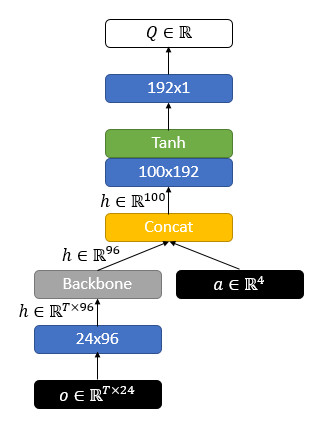
\includegraphics[width=0.9\linewidth]{figures/nets/critic.png}
		\caption{Critic Architecture}
		\label{fig:critic_net}
	\end{subfigure}
	\begin{subfigure}{.35\textwidth}
		\centering
		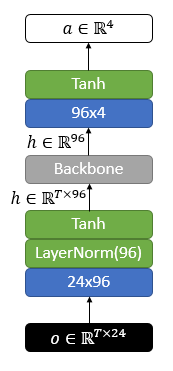
\includegraphics[width=0.6\linewidth]{figures/nets/actor.png}
		\caption{Actor Architecture}
		\label{fig:actor_net}
	\end{subfigure}
	\caption{Neural Architecture Design}
	\label{fig:nets}
\end{figure}

As backbones, following networks are proposed. 

\subsubsection{Residual Feed Forward Network}

As Feed Forward Networks becomes deeper, optimizing weights gets difficult. 
Therefore, people come with the idea of residual connections~\cite{he_deep_2015}. 
For a fixed number of stacked layers (usually 2 which is single skip), input and output of the stack is summed up for next calculations. 
Replacing feed forward layers with other types yield different kind of residual network. 
The difference is demonstrated in Figure \ref{fig:rffnn_ffnn}.
Yellow blocks are layers where $\phi$ indicates layer has activation while empty ones are linear layers.

\begin{figure}
	\centering
	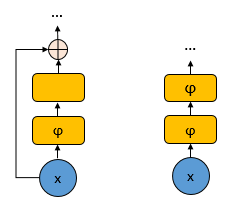
\includegraphics[width=0.5\textwidth]{figures/ml_theory/rffnn_vs_ffnn.png}
	\caption{Deep Feed Forward (left) and Deep Residual Feed Forward Network with single skip connection (right)}
	\label{fig:rffnn_ffnn}
\end{figure}

In our application, incoming vector is passed through 2 layers with 192 dimensional hidden size and 96 dimensional output with single skip connection, where there is GELU activation at first layer. 
 
\subsubsection{Long Short Term Memory}

Long Short Term Memory (LSTM)~\cite{hochreiter_long_1997} is a special type of Recurrent Neural Network. 
It is explicitly designed to allow learning long-term dependencies~\cite{olah_understanding_2015}. 
A single LSTM cell has 4 neural layer while vanilla RNN layer has only one neural layer. 
In addition to hidden state $h_t$, there is another state called cell state $C_t$. 
Information flow is controlled by 3 gates. 

\begin{figure}
	\centering
	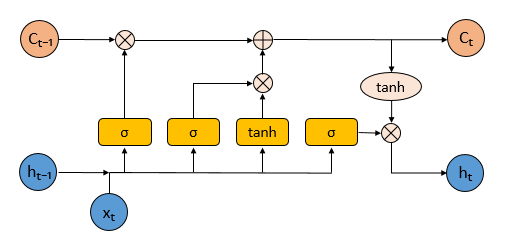
\includegraphics[width=0.85\textwidth]{figures/ml_theory/lstm_cell.png}
	\caption{LSTM Cell}
	\label{fig:lstm_cell}
\end{figure}

In our application, sequence of incoming vectors is passed though single vanilla LSTM layer with 96 dimensional hidden state. 
Output at last time step is considered as belief state. 

\subsubsection{Transformer (Pre-layer Normalized)}

The Transformer was proposed in Attention is All You Need~ \cite{vaswani_attention_2017} paper. 
Unlike recurrent networks, this architecture is solely builded on attention layers. 
However, original transformer architecture includes layer normalization operations after attention and feed-forward layers. 
It is unstable since the values of gradients of output layers are high, so Pre-Layer Normalized transformer is proposed by \cite{xiong_layer_2020} by carrying layer normalization operation to in front of attention and feed-forward layers. 
Moreover, Parisotto et al. Xiong et al.~ \cite{parisotto_stabilizing_2019} proposed gated transformer which also includes layer normalizations before attention and feedforward layer. 
They also stated that although gated architecture improves many RL tasks drastically, non-gated pre-layer normalized transformer are good enough. 
A simple pre-layer normalized transformer encoder layer is demonstrated in Figure \ref{fig:pre_trsf}.

\begin{figure}
	\centering
	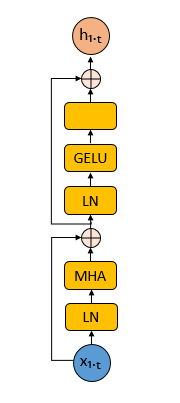
\includegraphics[width=0.3\textwidth]{figures/ml_theory/transformer_block.png}
	\caption{Pre-LN Transformer encoder layer with GELU activation}
	\label{fig:pre_trsf}
\end{figure}

In our application, sequence of incoming vectors is passed through single pre-layer normalized transformer layer with 192 dimensional feed forward layer with GELU activation. 
In multi-head attention, 4 head is used and size of queris, keys and values are 8 for each head.
During multi-head attention, only the last observation is fed as query so that attentions are calculated only for last state.  
Its output is considered as belief state.
Note that excluding multi-head attention for this network gives our residual feed-forward neural network.

\subsection{Algorithm Settings}
TD3 and SAC is used as RL algorithm. 
All hyperparameters are found after a trial-error process considering the literature. Adam optimizer is used for optimization. 
For all models, agents are trained by 8000 episodes.

In TD3, as exploration noise, Ornstein-Uhlenbeck noise is used, and standart deviation is multiplied  by $0.9995$ at the end of each episode. For LSTM and Transformer, last 6 observations are used to train agent. 

In SAC model, squashed gaussian policy is implemented. 
Therefore, along with layer giving mean actions, an additive layer is implemented for standart deviation along with it. 
For LSTM and Transformer, last 6 observations and 12 observations are used to train agent. 

Training sessions are run by multiple times to make comparison fair among models since some training sessions fail to converge and some yield worse results.

\subsection{Results and Discussion}

For each episode, episode scores are calculated by summing up rewards of each time step. 
In Figure \ref{fig:td3_std_ep_rewards} and Figure \ref{fig:sac_std_ep_rewards}, moving average and standard deviation is visualized for each model's episode scores. 

\begin{figure}[!ht]
	\centering
	\begin{subfigure}{.49\textwidth}
		\centering
		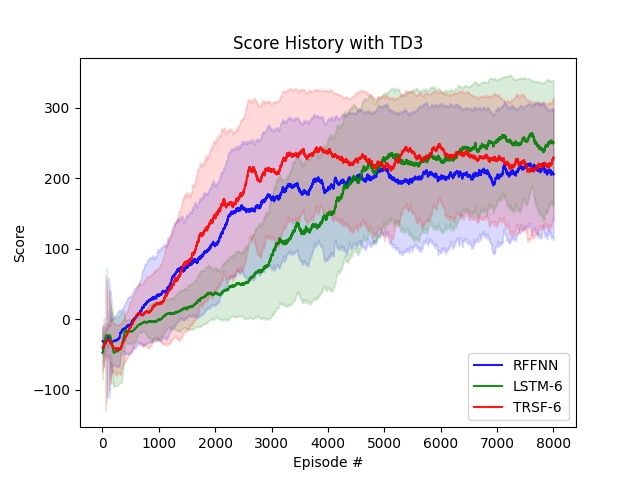
\includegraphics[width=0.99\textwidth]{figures/bipedal/STD_TD3_RFFNN_LSTM-6_TRSF-6.png}
		\caption{TD3}
		\label{fig:td3_std_ep_rewards}
	\end{subfigure}
	\begin{subfigure}{.49\textwidth}
		\centering
		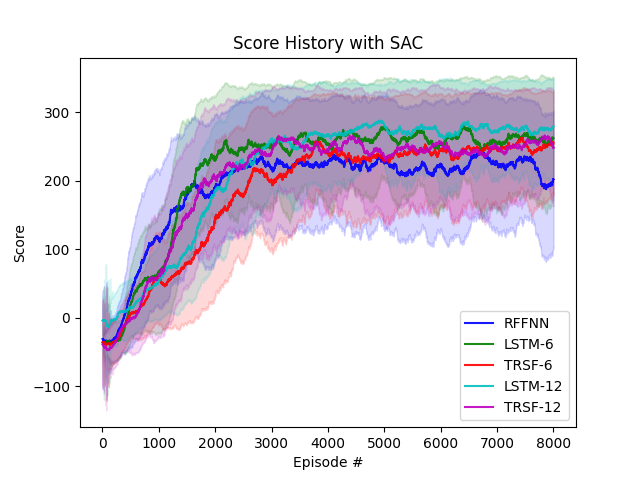
\includegraphics[width=0.95\textwidth]{figures/bipedal/STD_SAC_RFFNN_LSTM-6_TRSF-6_LSTM-12_TRSF-12.png}
		\caption{SAC}
		\label{fig:sac_std_ep_rewards}
	\end{subfigure}
	\caption{Moving Average and Standard Deviation for Episode Scores (Window length: 200 episodes) for TD3}
\end{figure}

RFFNN seems enough to make agent walk, although there exist partial observability in the environment. 
That model reaches around 221 points in average with TD3 and 245 points with SAC. 

Transformer models yield better performance compared to RFFNN. 249 points are reached by TD3 and 262 points reached by SAC model when 6 last observations are fed to the model. 266 points are obtained when last 12 observations are fed to model with SAC.

LSTM model yield the best results by reaching 264 points with TD3 and exceeds 280 points with SAC when 6 last observations are fed to model. 287 points are obtained when last 12 observations are fed to the model with SAC. 

These scores are maximum obtained average scores of concurrent 200 episodes during training. 
However, while traning, model changes and agent still tries to explore envrionment. 
Officially, 300 points in average required in random 100 simulations to say the environment is solved~\cite{noauthor_gymleaderboard_2021}.
Therefore, best checkpoints are evaluated for 100 concurrent simulations without exploration. 
Results are summarized in Table \ref{table:ckpt_performance}.

\begin{table}
	\begin{center}
		\caption{Best checkpoint performances with 100 test simulations}
		\begin{tabular}{||c c c c||} 
			\hline
			RL Method & Model & Episode & Avg. Score \\ [0.5ex] 
			\hline\hline
			TD3 & RFFNN & 6600 & 207 \\ 
			\hline
			SAC & RFFNN & 7600 & 219 \\
			\hline
			TD3 & TRSF-6 & 6400 & 222 \\
			\hline
			SAC & TRSF-6 & 6800 & 254 \\
			\hline
			SAC & TRSF-12 & 6000 & 270 \\
			\hline
			TD3 & LSTM-6 & 7000 & 242 \\
			\hline
			SAC & LSTM-6 & 7600 & 268 \\
			\hline
			SAC & LSTM-12 & 7200 & 298 \\ [1ex] 
			\hline
		\end{tabular}
		\label{table:ckpt_performance}
	\end{center}
\end{table}

None of our models exceed 300 point limit, but LSTM-12 model with SAC almost reaches to the limit Figure \ref{table:ckpt_performance}. 
However, all models partially solved problems by exceeding 200 point limit, while some simulations exceed 300 points with both TD3 (Figure \ref{fig:td3_stdr_ep_rewards}) and SAC (Figure \ref{fig:sac_std_ep_rewards}). 

Behaviour of agents are visualized in Figure \ref{fig:rffnn_simulation}, Figure \ref{fig:lstm_simulation} and Figure \ref{fig:trsf_simulation} for SAC models. 
All of 3 models exhibit similar walking characteriscis.

SAC model performes better than TD3 in general, as seen in Figure \ref{fig:td3_std_ep_rewards} and Figure \ref{fig:sac_std_ep_rewards}. 
In addition, as seen from the moving average points, SAC agents are superior (Figure \ref{fig:td3_std_ep_rewards}, Figure \ref{fig:sac_std_ep_rewards}).

\begin{figure}[!ht]
	\centering
	\begin{subfigure}{.95\textwidth}
		\centering
		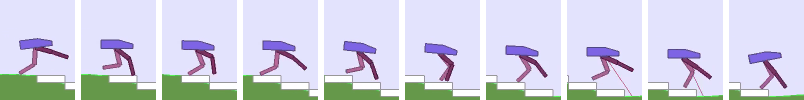
\includegraphics[width=0.95\textwidth]{figures/bipedal/anim/ff-stairs.png}
		\caption{Stairs}
		\label{fig:anim_rffnn_stairs}
	\end{subfigure}
	\begin{subfigure}{.95\textwidth}
		\centering
		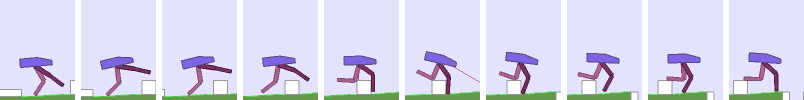
\includegraphics[width=0.95\textwidth]{figures/bipedal/anim/ff-hurdle.png}
		\caption{Hurdle}
		\label{fig:anim_rffnn_hurdle}
	\end{subfigure}
	\begin{subfigure}{.95\textwidth}
		\centering
		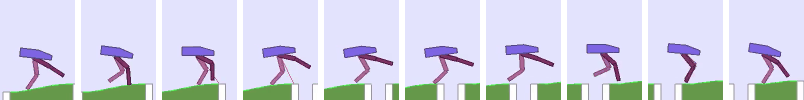
\includegraphics[width=0.95\textwidth]{figures/bipedal/anim/ff-pitfall.png}
		\caption{Pitfall}
		\label{fig:anim_rffnn_pitfall}
	\end{subfigure}
	\caption{Walking Simulation of RFFNN model at best version with SAC}
	\label{fig:rffnn_simulation}
\end{figure}

\begin{figure}[!ht]
	\centering
	\begin{subfigure}{.95\textwidth}
		\centering
		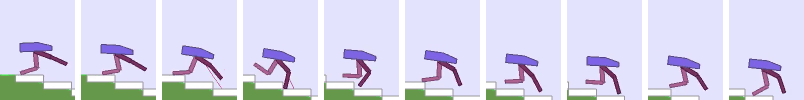
\includegraphics[width=0.95\textwidth]{figures/bipedal/anim/lstm-12-stairs.png}
		\caption{Stairs}
		\label{fig:anim_lstm_stairs}
	\end{subfigure}
	\begin{subfigure}{.95\textwidth}
		\centering
		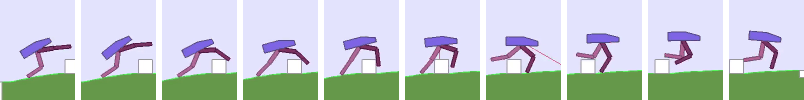
\includegraphics[width=0.95\textwidth]{figures/bipedal/anim/lstm-12-hurdle.png}
		\caption{Hurdle}
		\label{fig:anim_lstm_hurdle}
	\end{subfigure}
	\begin{subfigure}{.95\textwidth}
		\centering
		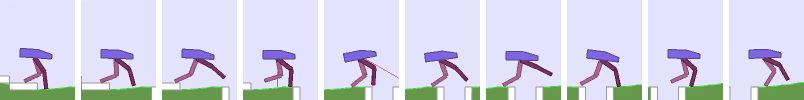
\includegraphics[width=0.95\textwidth]{figures/bipedal/anim/lstm-12-pitfall.png}
		\caption{Pitfall}
		\label{fig:anim_lstm_pitfall}
	\end{subfigure}
	\caption{Walking Simulation of LSTM-12 model at best version with SAC}
	\label{fig:lstm_simulation}
\end{figure}

\begin{figure}[!ht]
	\centering
	\begin{subfigure}{.95\textwidth}
		\centering
		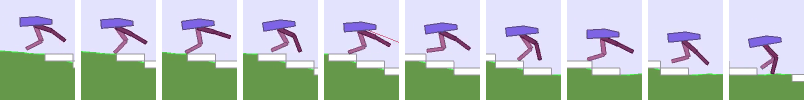
\includegraphics[width=0.95\textwidth]{figures/bipedal/anim/trsf-12-stairs.png}
		\caption{Stairs}
		\label{fig:anim_trsf_stairs}
	\end{subfigure}
	\begin{subfigure}{.95\textwidth}
		\centering
		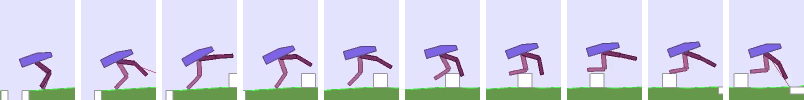
\includegraphics[width=0.95\textwidth]{figures/bipedal/anim/trsf-12-hurdle.png}
		\caption{Hurdle}
		\label{fig:anim_trsf_hurdle}
	\end{subfigure}
	\begin{subfigure}{.95\textwidth}
		\centering
		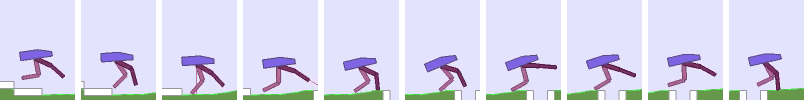
\includegraphics[width=0.95\textwidth]{figures/bipedal/anim/trsf-12-pitfall.png}
		\caption{Pitfall}
		\label{fig:anim_trsf_pitfall}
	\end{subfigure}
	\caption{Walking Simulation of Transformer-12 model at best version with SAC}
	\label{fig:trsf_simulation}
\end{figure}

%%% DISCUSSION %%%
%%%%%%%%%%%%%%%%%%
We believe that these results are not enough to conclude on a superior neural network for all RL problems, because there are other factors such as DRL algorithm, number of episodes, network size etc. 
However, networks are designed to have similar sizes and good model requires to converge in less episodes. 
As a result, LSTM is superior to Transformer for our environment. 
In addition, it is possible to conclude that Transformers can be on aoption for partially observed RL problems, thanks to incorprating observation history. 
Note that this is valid where layer normalization is applied before multihead attention and feed-forward layers \cite{xiong_layer_2020} as opposed to vanilla transformer proposed in \cite{vaswani_attention_2017}. 

Another result is that incorprating past observations did improve performance significantly since environment is partially observable.
Especially increasing history length keep increasing performance for both LSTM and Transformer models. 

The environment is a difficult one. 
There are really few available models which gets close to a solution. 
Apart from neural networks, there are other factors affecting performance such as RL algorithm, rewarding, exploration etc. 
In this work, all of them are adjusted such that the environment becomes solvable. 
Time frequency is reduced for sample efficiency and speed. 
Also, the agent is not informed for the terminal state when it reaches time limit. 
Those modifications seems to be behind getting close to a solution. 
Lastly, punishment of failing reduced, so the agent is allowed to learn by mistakes. 
We believe that those modifications are also source of our high performance. 

As RL algorithm, TD3 is selected first, since it is a good choice for continuous RL. 
Ornstein-Uhlenbeck noise is used for better exploration since it has momentum, and its variance is reduced by time to make agent learn small actions well in later episodes. 
In addition, SAC is used for learning along with TD3. 
Results are better compared to those of TD3. 
SAC policy maximizes randomness (entropy) if agent cannot get sufficient reward and this allows the agent to decide where/when to explore more or less. 
This way, SAC handles the sparse rewards from the environment better than TD3. 

\section{Conclusion}

For robot control by RL in real world, simulation is an important step. 
Usually, models are pretrained in simulation environment before learning in reality due to safety and exploration reasons. 
Today, RL is rarely used in real world applications due to safety and sample inefficiency problems. 

In this thesis, bipedal robot walking is investigated by deep  reinforcement learning due to complex dynamics in OpenAI Gym's simulation environment. 
TD3 and SAC algorthims are used since they are robust and well suited for continuous control. 
Also, environment is slightly modified by reward shaping, halving simulation frequency, cancelling terminal state information at time limit so that learning becomes easier.

As stated in previous chapters, most of the real world environments are partially observable. 
In BipedalWalker-Hardcore, the environment is also partially observable since agent cannot observe behind and it lacks of acceleration sensors, which is better to have for controlling mechanical systems. 
Therefore, we propose to use Long Short Term Memory (LSTM) and Transformer Neural Networks to capture more information from past observations unlike Residual Feed Forward Neural Network (RFFNN) using a single instant observation as input. 

RFFNN model performed well thanks to carefully selected hyperparameters and modifications on the environment. 
However, sequential models performed much better indicating partial observability is an important issue for our environment. 
Among sequential models, LSTM performed better compared to Transformer agents. 

Another conclusion is that transformer model worked enough to say it can be used in DRL problems. 
It is surprising because it is not succesfully used in DRL problems in general except recent architectural developments~\cite{parisotto_stabilizing_2019}. 
In natural language processing, this type of attention models completely replace recurrent models recently, and our results seems promising for this in DRL domain. 

The environment was difficult for exploration. 
Especially handling big hurdles requires very much exploration.
In our results, SAC agents performed better than TD3 since it handles exploration problem by learning how much to explore for a particular state. 

\section{References}

%%%%%%%%%%%%%%%%%%%%%%%%%%%%
% CONTENT ENDS HERE (almost)
%%%%%%%%%%%%%%%%%%%%%%%%%%%%



%%% The following way of Bibliography is not recommended
%\begin{thebibliography}{99}
	%\bibitem{bertcs96}  G. Berkooz,  P. Holmes and  J.L.  Lumley.
  %Turbulence, Coherent Structuress, Dynamical Systems and Symmetry,
  %Cambridge University Press: Cambridge Monographs on Mechanics,
  %1996. 
%
	%\bibitem{fukisr90}  K. Fukunaga. Introduction to statistical pattern
  %recognition. Computer Science and Scientific Computing. 
	%Academic Press Inc., Boston, MA, second edition, 1990.
%\end{thebibliography}

%
% References in Bibtex format goes into below 
% indicated file with .bib extension
\bibliography{myBiblio} % filename: myBiblio.bib
% You can use full name of authors, 
% however most likely some of the Bibtex entries you will find, 
% will use abbreviated first names.
% If you don't want to correct each of them by hand, 
% you can use abbreviated style for all of the references
% \bibliographystyle{abbrv}
% However, IAM suggests to use
\bibliographystyle{iamBiblioStyle} % better than to use {plain or abbrv}

%%% APPENDIXES in case you need
%\appendix
%
% input your appendix
% If you are not using minted style, then comment the first appendix below
% otherwise uncomment.
%uncomment%  \chapter{Proof of Some Theorem}
\label{app:mintedCodes}

This is appendix text.

\definecolor{myBgColour}{rgb}{0.99,0.99,0.99} % almost white

\setminted[python]{frame=single,
framesep=2mm,
baselinestretch=1.1,
bgcolor=myBgColour,
fontsize=\footnotesize,
linenos, autogobble,
python3=true}

\setminted[matlab]{frame=single,
framesep=2mm,
baselinestretch=1.1,
bgcolor=myBgColour,
fontsize=\footnotesize,
linenos, autogobble,
python3=true}

%\captionsetup[Listing]{format=plain,font={small},labelfont={bf}, aboveskip=-5px}
%\renewcommand{\theListing}{{\arabic{Listing}}}
%\setcounter{Listing}{0}


However, we place a python code here with a listing environment
Listing~\ref{lst:first}.	

\begin{listing}	
\begin{minted}{python}
# Python program to check if the input number is prime or not

num = 407

# take input from the user
# num = int(input("Enter a number: "))

# prime numbers are greater than 1
if num > 1:
   # check for factors
   for i in range(2,num):
       if (num % i) == 0:
           print(num,"is not a prime number")
           print(i,"times",num//i,"is",num)
           break
   else:
       print(num,"is a prime number")
       
# if input number is less than
# or equal to 1, it is not prime
else:
   print(num,"is not a prime number")
\end{minted}
\caption{This is the caption of this Listing environment\label{lst:first}}
\end{listing}

Also we wish to insert a MATLAB code, too.

\definecolor{myBackgroundColour}{rgb}{0.9,0.9,0.9} % almost gray
\begin{minted}[
frame=lines,
framesep=2mm,
baselinestretch=1.2,
bgcolor=myBackgroundColour,
fontsize=\footnotesize,
linenos
]{matlab}
function result = myprime(n)
% MATLAB program to check if the input number is prime or not

%% initially set output flag to true
 result = true;
%% iterate over all positive integers 2,3,...,n-1
%% if n is not divisible by any of these factors....it is prime
 if (n == 1)
     result = 'false';
 elseif (n == 2)
     result = 'true';
 else 
    for i=2:n-1,
        if (mod(n,i)==0)
           result = 'false';
        end
    end
 end
%% return "true" or "false" instead of 1 or 0  
 if (result)
    result = 'true';
 else
    result = 'false';
 end
\end{minted}


Furthermore, here are two files (myPythonCode.py and myMatlabCode.m) included.

\inputminted[
frame=single,
framesep=2mm,
baselinestretch=1.2,
bgcolor=myBackgroundColour,
fontsize=\footnotesize,
linenos
]{python}{myPythonCode.py}

\definecolor{myRed}{rgb}{0.95,0.1,0.1}

\begin{listing}
\inputminted[frame=single, linenos, bgcolor=myRed]{matlab}{myMatlabCode.m}
\caption{Here is the caption again}
\end{listing} % includes minted package examples!
%\chapter{Proof of Some Theorem}
\label{app:somethms}

This is appendix text.

\begin{listing}
  %\VerbListingBoxed{myMatlabCode.m}
  \VerbatimInput{myMatlabCode.m}
	%\inputminted{matlab}{myMatlabCode.m} % only if minted is used!
  %\VerbListing{myMatlabCode.m}
\caption{The \texttt{lintest} function in a floating ``listing'' environment.}
\label{mfile:linetest-3}
\end{listing}




\end{document}

